\chapter{MDPs}

What is a decision problem?
Why do we care?

\hypertarget{sequential-decision-problems}{%
\subsection{Sequential decision
problems}\label{sequential-decision-problems}}

A MDP is defined as a tuple, \(\{\mathcal S, \mathcal A, P(s_{t+1} \mid s_t, a_t),R(s_t, a_t, s_{t+1}), \gamma\}\)\footnotemark[1]. Where \(s \in \mathcal S\) is the set of possible states (\textit{for example arrangements of chess pieces}), \(a \in \mathcal A\) is the set of actions (\textit{the different possible moves, left, right, diagonal, weird L-shaped thing, ...}),  \(P(s_{t+1} \mid s_t, a_t)\) is the transition function which describes how the environment acts in response to the past (\(s_t\)) and to your actions (\(a_t\)) (\textit{in this case, your opponent's moves, taking one of your pieces, and the results of your actions}), and finally, \(r(s_t, a_t, s_{t+1})\) is the reward function, \textit{whether you won (+1) or lost (-1) the game}) and \(R ={\sum_{t=0}}^T r(s_t, a_t, s_{t+1}) \) is the cumulative reward, or return. The player's goal, is to learn a policy \(\pi\), (which chooses actions, \(a_t = \pi(s_t)\)) that yields the largest return \(\text{max } R\).

\footnotetext[1]{Why is the discount factor a part of the definition of the MDP?
By defining the discount it ensures the MDP has a unique solution.}

If we wanted we could pick our actions before we make observations,
reducing the search space to only \(|A| \times T\). But this is a bad idea\ldots{} example.

\hypertarget{mdps}{%
\subsection{Related settings}\label{mdps}}

\begin{itemize}
\tightlist
\item
  Observable
\item
  Deterministic
\item
  Synchronous
\item
  Terminating
\item
  Knowledge of the model
\item
  Discrete
\end{itemize}

MDPs are a subset of sequential decision problem. Define MDPs. Give
example.

When actions you have taken in the past can bite you in the butt \ldots{}
Maze with pendulums / doors. When moving through the maze, you must
swing the pendulums. In the future you must avoid being hit. (maybe make
a picture of this?) also, is there a more general way to think about it?

The general feeling of an MDP. - Actions need to be adapted to new
observations and contexts. - While instantaneous results are good, we
care about the longer term aggregates.

\begin{align*}
Q^{\pi}(s_0, a_0) = r(s_0, a_0)
+ \gamma \mathop{\text{max}}_{a_1} \mathop{\mathbb E}_{s_1\sim p(\cdot | s_0, a_0)} \Bigg[ r(s_1, a_1) \\
+ \gamma \mathop{\text{max}}_{a_2} \mathop{\mathbb E}_{s_2\sim p(\cdot | s_1, a_1)} \bigg[r(s_2, a_2)
+ \gamma \mathop{\text{max}}_{a_3} \mathop{\mathbb E}_{s_3\sim p(\cdot | s_2, a_2)} \Big[
\dots \Big] \bigg] \Bigg]
\end{align*}

\hypertarget{the-markov-property}{%
\subsubsection{The Markov property}\label{the-markov-property}}

What does the M in MDP mean?

When we say a decision problem is Markovian, we mean that the transition
function acts as a Markov chain. The next transition step depends only
on the current state. It is invariant to any / all histories that do not
change the current state.

This is not to say that past actions do not effect the future. Rather,
it is a special type of dependence on the past. Where the dependence is
totally described by changes to the \textbf{observable} state.

Can easily make a sequence Markovian by adding information. E.g.
time

\hypertarget{optimality}{%
\subsubsection{Optimality}\label{optimality}}

And importantly, existing theory tells us that there is a unique optima to the bellman iterations.
And that this optimal policy(ies) is(are) necessarily deterministic.


(why does this make sense?)

\hypertarget{how-do-mdps-relate-to-rl}{%
\subsubsection{How do MDPs relate to RL?}\label{how-do-mdps-relate-to-rl}}

Reinforcement learning referces to the set of solutions to a type of problem.
This general, reinforcement learning, problem, has two main properties;
"trial-and-error search and delayed rewards" [@Sutton1998ReinforcementLA].
Unlike supervised learning, which gives the learner feedback (\textit{I think that digit
is a 5 -> no, it's a 6}), in RL the learner only receives evaluations (\textit{I think
that digit is a 5 -> wrong}). Ontop of terse teachers, many actions may be taken
before any evaluation is received, thus requiring credit to be assigned to actions,
often leaving the learner wondering: "what did I do to deserve this?" (see
[pigeon superstition](https://www.youtube.com/watch?v=8uPmeWiFTIw) for an amusing
example of credit assignment gone wrong [@Skinner1948SuperstitionIT]).

MDPs are also within the fields of Operational Research, Optimal Control, Mathematical
Optimisation, Stochastic Programming.

\hypertarget{a-tabular-representation-of-mdps}{%
\subsubsection{A tabular representation of MDPs}\label{a-tabular-representation-of-mdps}}

Tabular MDPs with deterministic actions are of little interest to the ML
community. Not because they are easy, but because they can be solved by non-statistical
methods: dynamic programming and related planning techniques.

The minimally complex MDP that poses an interesting challenge to the ML
community is when the transition function is non deterministic.

Just quickly, what does a tabular MDP look like? We iscrete states and
actions - \(r\) and \(P\) are simply look up functions, indexed by the
current state-action.

A result of this formulation is that we consisely write and solve the Bellman equation.

\begin{align}
V &= r_{\pi} + \gamma P_{\pi} V \tag{bellman eqn}\\
V - \gamma P_{\pi} V &= r_{\pi}\\
(I-\gamma P_{\pi})V &= r_{\pi}\\
V &= (I-\gamma P_{\pi})^{-1}r_{\pi}\\
\end{align}

\section{The value function polytope}

Why is it a polytope?
What are the value polytopes properties?

\begin{itemize}
\tightlist
\item
  Positive orthants
\item
  Straight sides
\item
  Non-convex
\end{itemize}

Imagine a two state MDP. Following some initial, ill-informed policy,
the value that you might get starting from each state is
${v_1}^0, {v_2}^0$.

An increase in the value of state one, can, at worst, do nothing for state two, aka a
flat line, either horizontal or vertical. This explains why the edges of the polytope by be
aligned with the positive orthant, they slant upward.


\begin{figure}
\centering
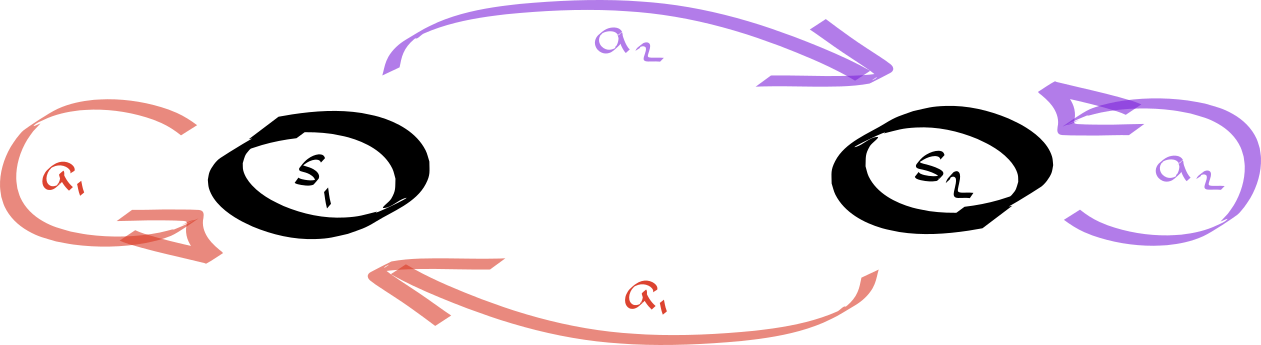
\includegraphics[width=1\textwidth,height=0.25\textheight]{../../pictures/drawings/2-state-automata.png}
\caption{Consider the simplest possible MDP, with two states and two actions. (Any simpler setting is uninteresting. A single state means actions do nothing.
And a single action means all policies are the same...).}
\end{figure}

\begin{figure}
\centering
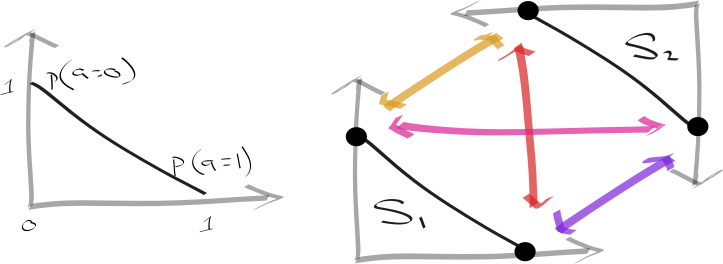
\includegraphics[width=1\textwidth,height=0.25\textheight]{../../pictures/drawings/2-state-2-action-simplices.png}
\caption{Imagine what the geometry of the space of policies in the two state, two action MDP. A policy tells us what actions should be taken when in a given state. Therefore, there will be \(|A| \times |S|\) entries in the policy. However, because the policy returns a distribution over actions, the true dimensionality of the policy is \((|A| -1) \times |S|\). Which in the two state, two action case equals 2D.}
\end{figure}

\begin{figure}
\centering
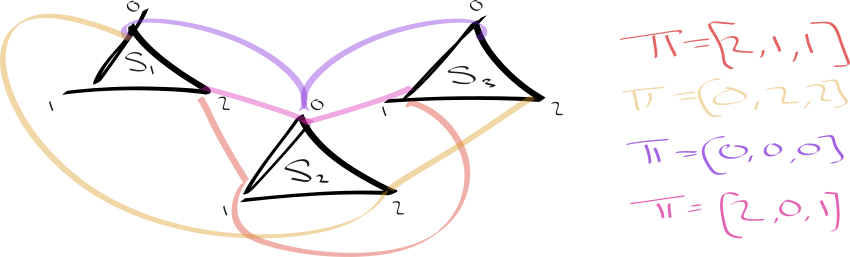
\includegraphics[width=1\textwidth,height=0.25\textheight]{../../pictures/drawings/3-state-3-action-simplices.png}
\caption{Let's \textit{try} to gain some intuition about the space of policies in higher dimensions.
For each state, we have a distribution (on a simplex), over the possible actions.}
\end{figure}

\begin{center}\rule{0.5\linewidth}{\linethickness}\end{center}

Some simple question to explore;

\begin{itemize}
\tightlist
\item
  What is the distribution of policies on the polytope?
\item
  How does the discount rate change the shape of the polytope?
\item
  How do the dynamics of GPI partition the policy / value spaces?
\end{itemize}

\subsection{Distribution of policies}

A potentially interesting question to ask about the polytopes is how the
policies are distributed over the polytope. To calculate this
analytically, we can use the probability chain rule:
\(p(f(x)) = \mid \det\frac{\partial f(x)}{\partial x}\mid^{-1}p(x)\).
Where we set \(f\) to be our value functional and \(p(x)\) to be a
uniform distribution.

\begin{figure}
\centering
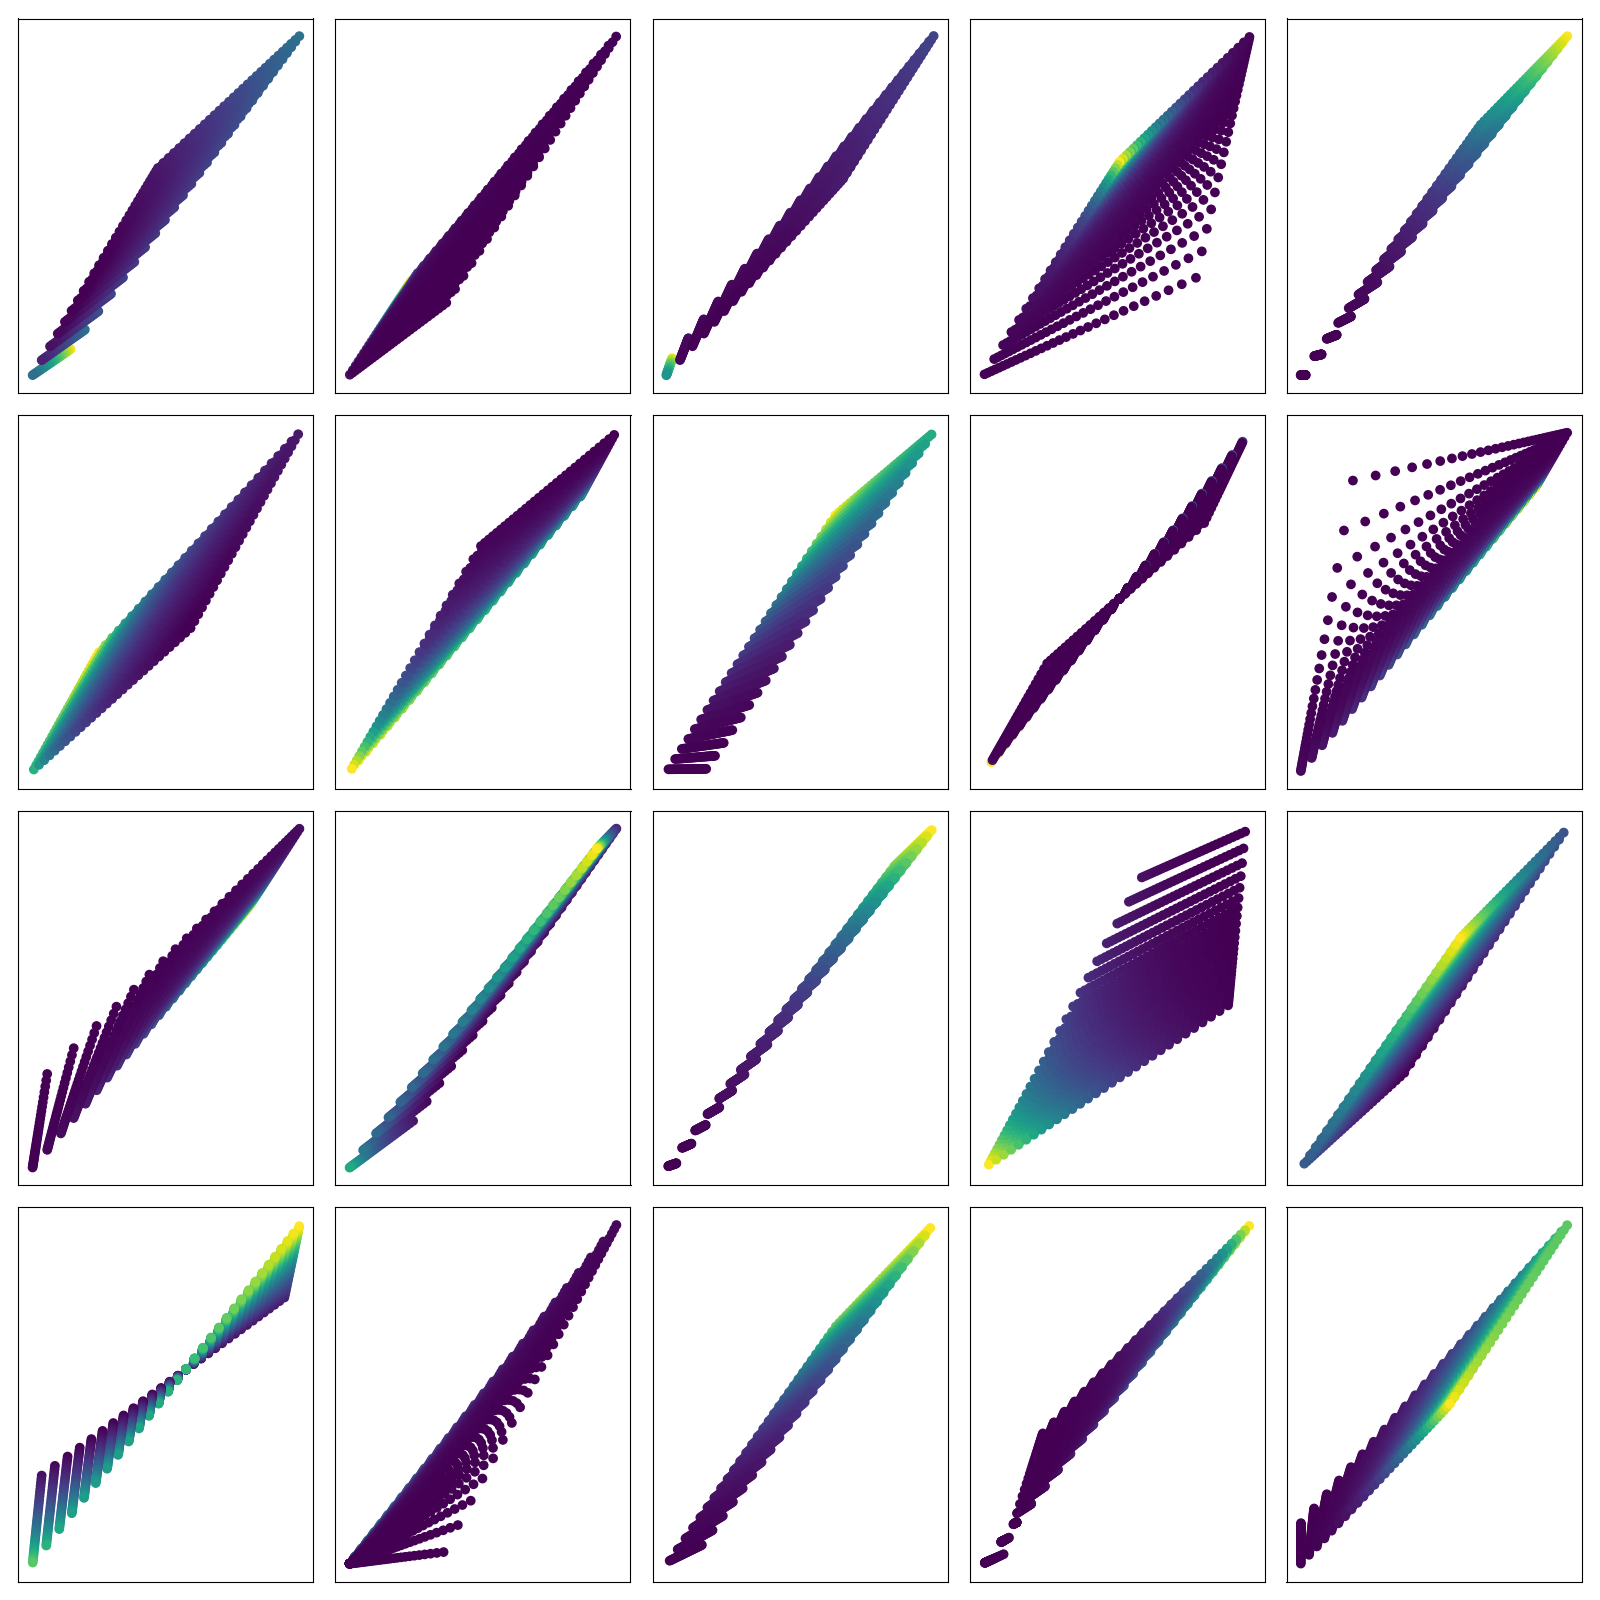
\includegraphics[width=0.5\textwidth,height=0.5\textheight]{../../pictures/figures/polytope_densities.png}
\caption{`2-state 2-action MDPs. We have visualised the likelihood of
values under a uniform on policies. They are coloured by density.
Lighter colour is higher probability'}
\end{figure}

\begin{itemize}
\item
  \textbf{Observation} In some polytopes, many of the policies are close
  to the optimal policy. In other polytopes, many of the policiesare far
  away from the optimal policy. \textbf{Question} Does this make the MDP
  harder or easier to solve? \textbf{Intuition} If there is a high
  density near the optimal policy then we could simply sample policies
  and evaluate them. This would allow us to find a near optimal policy
  with relative easy.
\item
  \textbf{Observation} The density is always concentrated / centered on
  an edge.
\item
  \textbf{Question} how does the entropy of the distribution change
  under different gamma/transitions/rewards\ldots{}?
\end{itemize}

\begin{center}\rule{0.5\linewidth}{\linethickness}\end{center}

\paragraph{An MDPs Entropy}

(\emph{the goal is to understand what makes some MDPs harder to solve
than others})

We can visualise polytopes in 2D, but we struggle in higher dimensions.
However, it is possible to use lower dimensions to gain intuition about
metrics and carry that intuition into higher dimensions. A potential
metric of interest here is the entropy of our distribution, (and / or
the expected distance from the optima) to give intuition about
unimaginable MDPs.

\begin{align}
M &\to \{P, r, \gamma\} \tag{a MDP}\\
H(M) &:= \mathop{\mathbb E}_{\pi\sim\Pi}\Big[-\log p(V(\pi)) \Big]\\
&= \mathop{\mathbb E}_{\pi\sim\Pi}\Big[-\log(\mid \det\frac{\partial V(\pi)}{\partial \pi}\mid^{-1}p(\pi)) \Big] \\
&= \mathop{\mathbb E}_{\pi\sim\Pi}\Big[-\log(\mid \det \frac{r}{(I-\gamma P \pi)^2}\mid^{-1}p(\pi)) \Big] \\
\end{align}

What does this tell us? \textbf{???} A MDP with a low entropy tells us
that many of the policies are in a corner of the polytope. But the
`hardness' of the MDP depends on which corner these policies are
concentrated in. Rather we could use the value of each policy to give
information about the location of the policy.

\begin{align*}
\mu(M) &:= \mathop{\mathbb E}_{\pi\sim\Pi}\Big[V(\pi) \Big]\\
\end{align*}

What does this tell us? The expected value of a policy. Thus, a quantity
of interest might be the expected suboptimality of a policy,
\(s = V(\pi^{* })-\mu(M)\). This tells us how far away the optimal
policy is from the center of mass of the polytope.

\textbf{Conjecture:} If an MDP has suboptimality
\(s \le \frac{\sigma_{MDP}}{D}\) then it is possible to find a
\(\epsilon\) optimal policy with \(\mathcal O(n)\) samples. (but
sampling in high dimensions always scales badly?!)

\textbf{Experiment:} Correlate the properties of \(P, r\) with entropy.
Or find derivative wrt \(P, r\). What properties of \(P, r\) yield
easily solvable MDPs?

NOTE:

\begin{itemize}
\item
  What about the variance of the MDP? What does that tell us?
\item
  How does a uniform distribution on a simplex behave in high
  dimensions? Does it become more likely to sample from the center? Less
  likely to sample from vertices??
\item
  In most cases, this is unlikely to work. A high dimensional polytope
  \ldots{} low density everywhere!?
\end{itemize}


\subsection{Discounting}

How does the shape of the polytope depend on the discount rate? Given an
MDP, we can vary the discount rate from \(0\) to \(1\) and explore how
the shape of the value polytope changes.

\begin{figure}
\centering
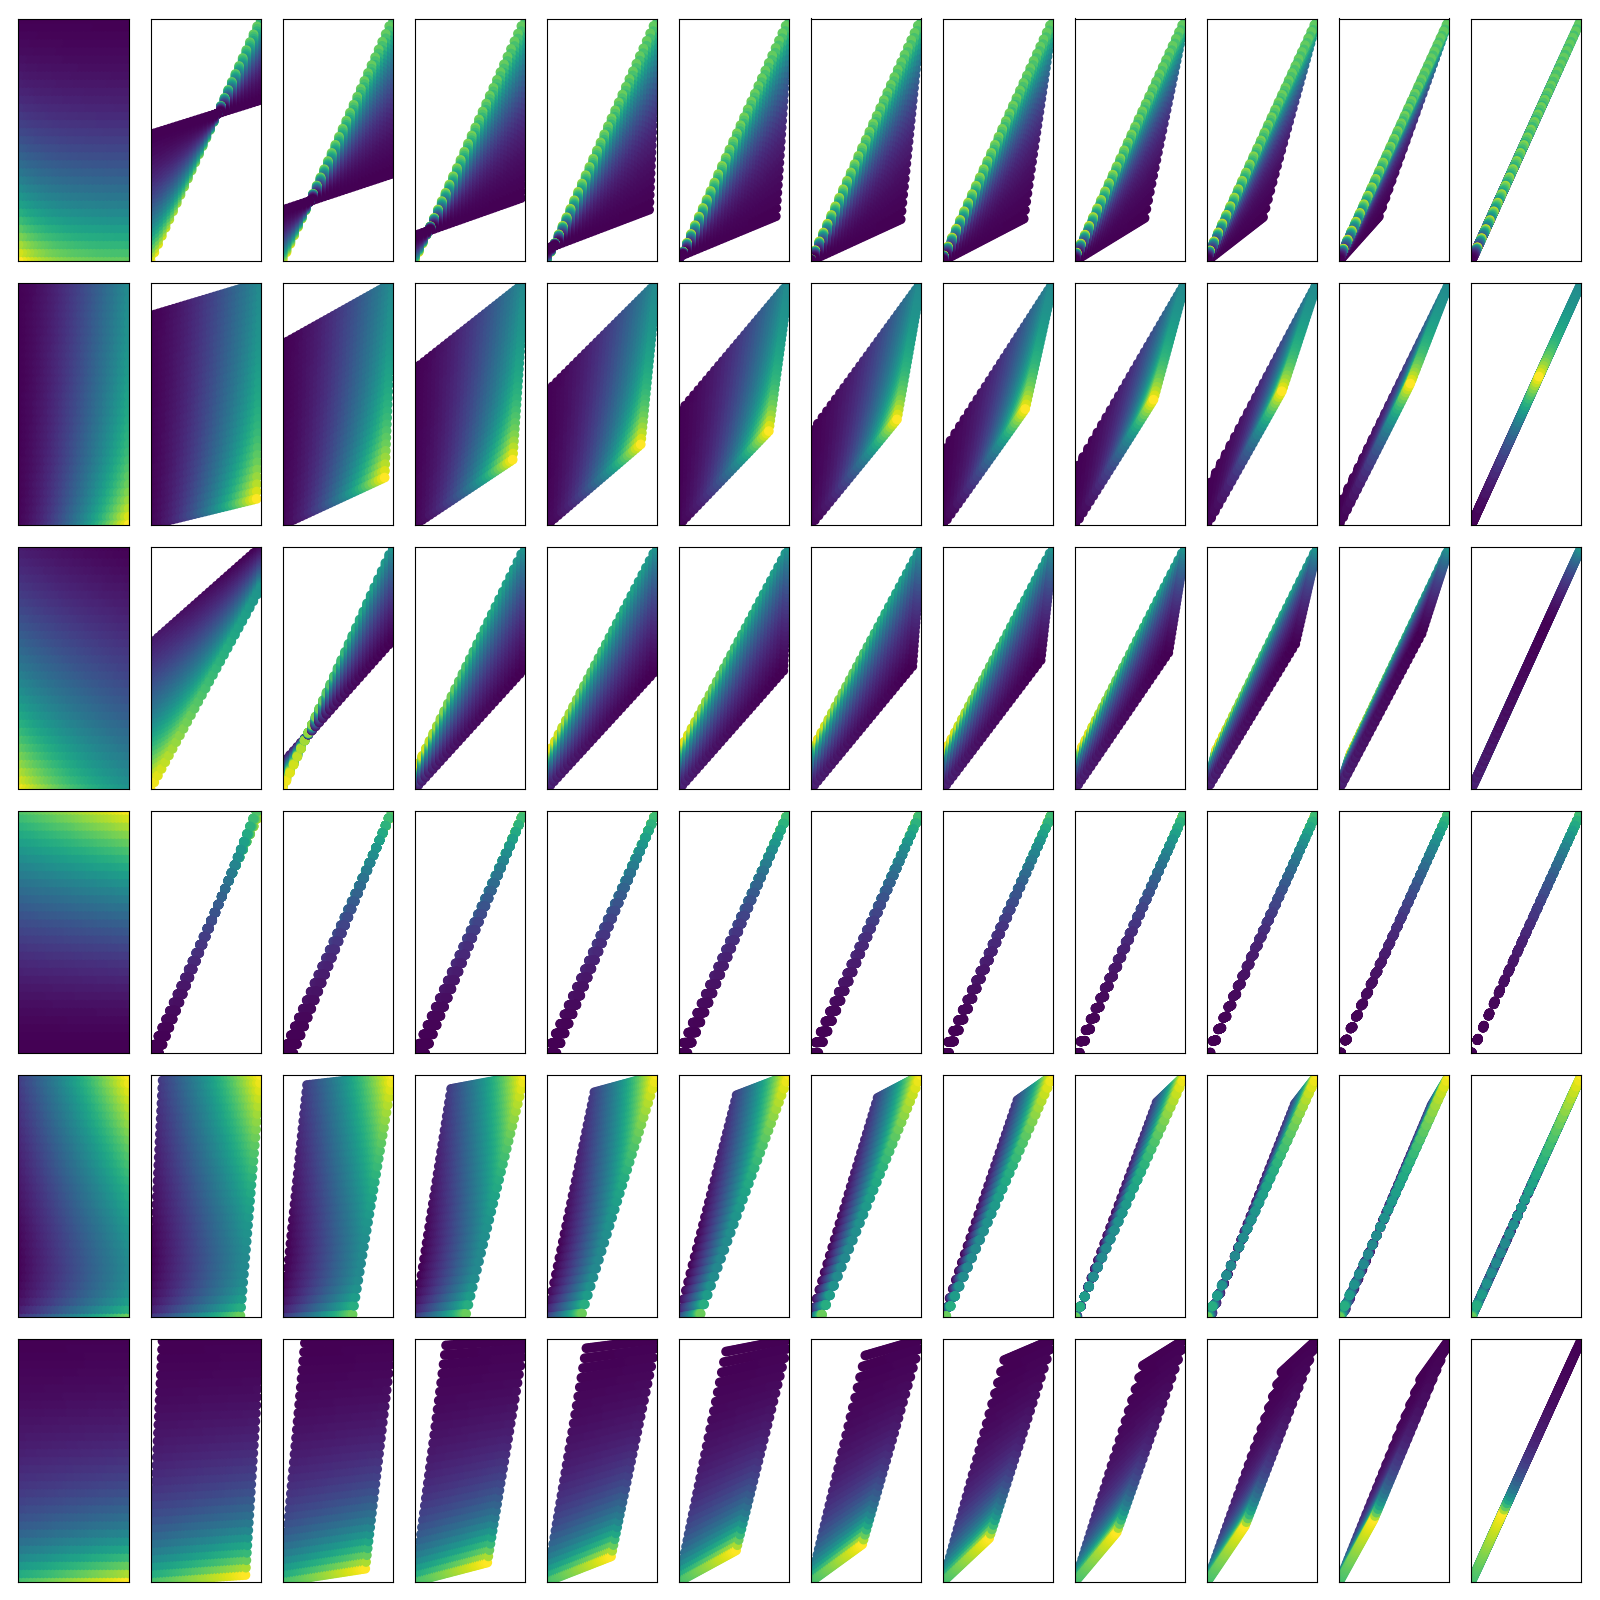
\includegraphics[width=0.5\textwidth,height=0.5\textheight]{../../pictures/figures/discounts.png}
\caption{`2-state 2-action MDPs. Here we have shown a few different P/r
MDPs and how their polytopes change with changes in discount rate.'}
\end{figure}

\begin{itemize}
\item
  \textbf{Observation} As \(\gamma \to 1\), all the policies are
  projected into a 1D space? \textbf{Question} Does this make things
  easier to learn? \textbf{Intuition} Orderd 1D spaces are easy to
  search.
\item
  \textbf{Observation} The tranformation that changing the discount
  applies is quite restricted. They are not generally non-linear, but
  appear `close to linear', but not quite. \textbf{Question} What is the
  set of functions /transformations that the discount can apply?
\end{itemize}

% ##############################################################################

\section{Search spaces}
\subsection{Dynamics and complexity}

\textbf{TODO} Complexity. How many iterations!!! Look up from literature
and do some empirical tests.

(we want to know how much it costs to find the optima)

For each initial policy, we can solve / optimise it to to find the
optimal policy (using policy iteration). Here we count how many
iterations were required to find the optima (from different starting
points / policies).

Policy iteration can be summarised easily as an iteration between
evaluation and updates, see below.

\begin{verbatim}
pi = init
while not converged:
  value = evaluate(pi)
  pi = greedy_update(value)
\end{verbatim}

\begin{figure}
\centering
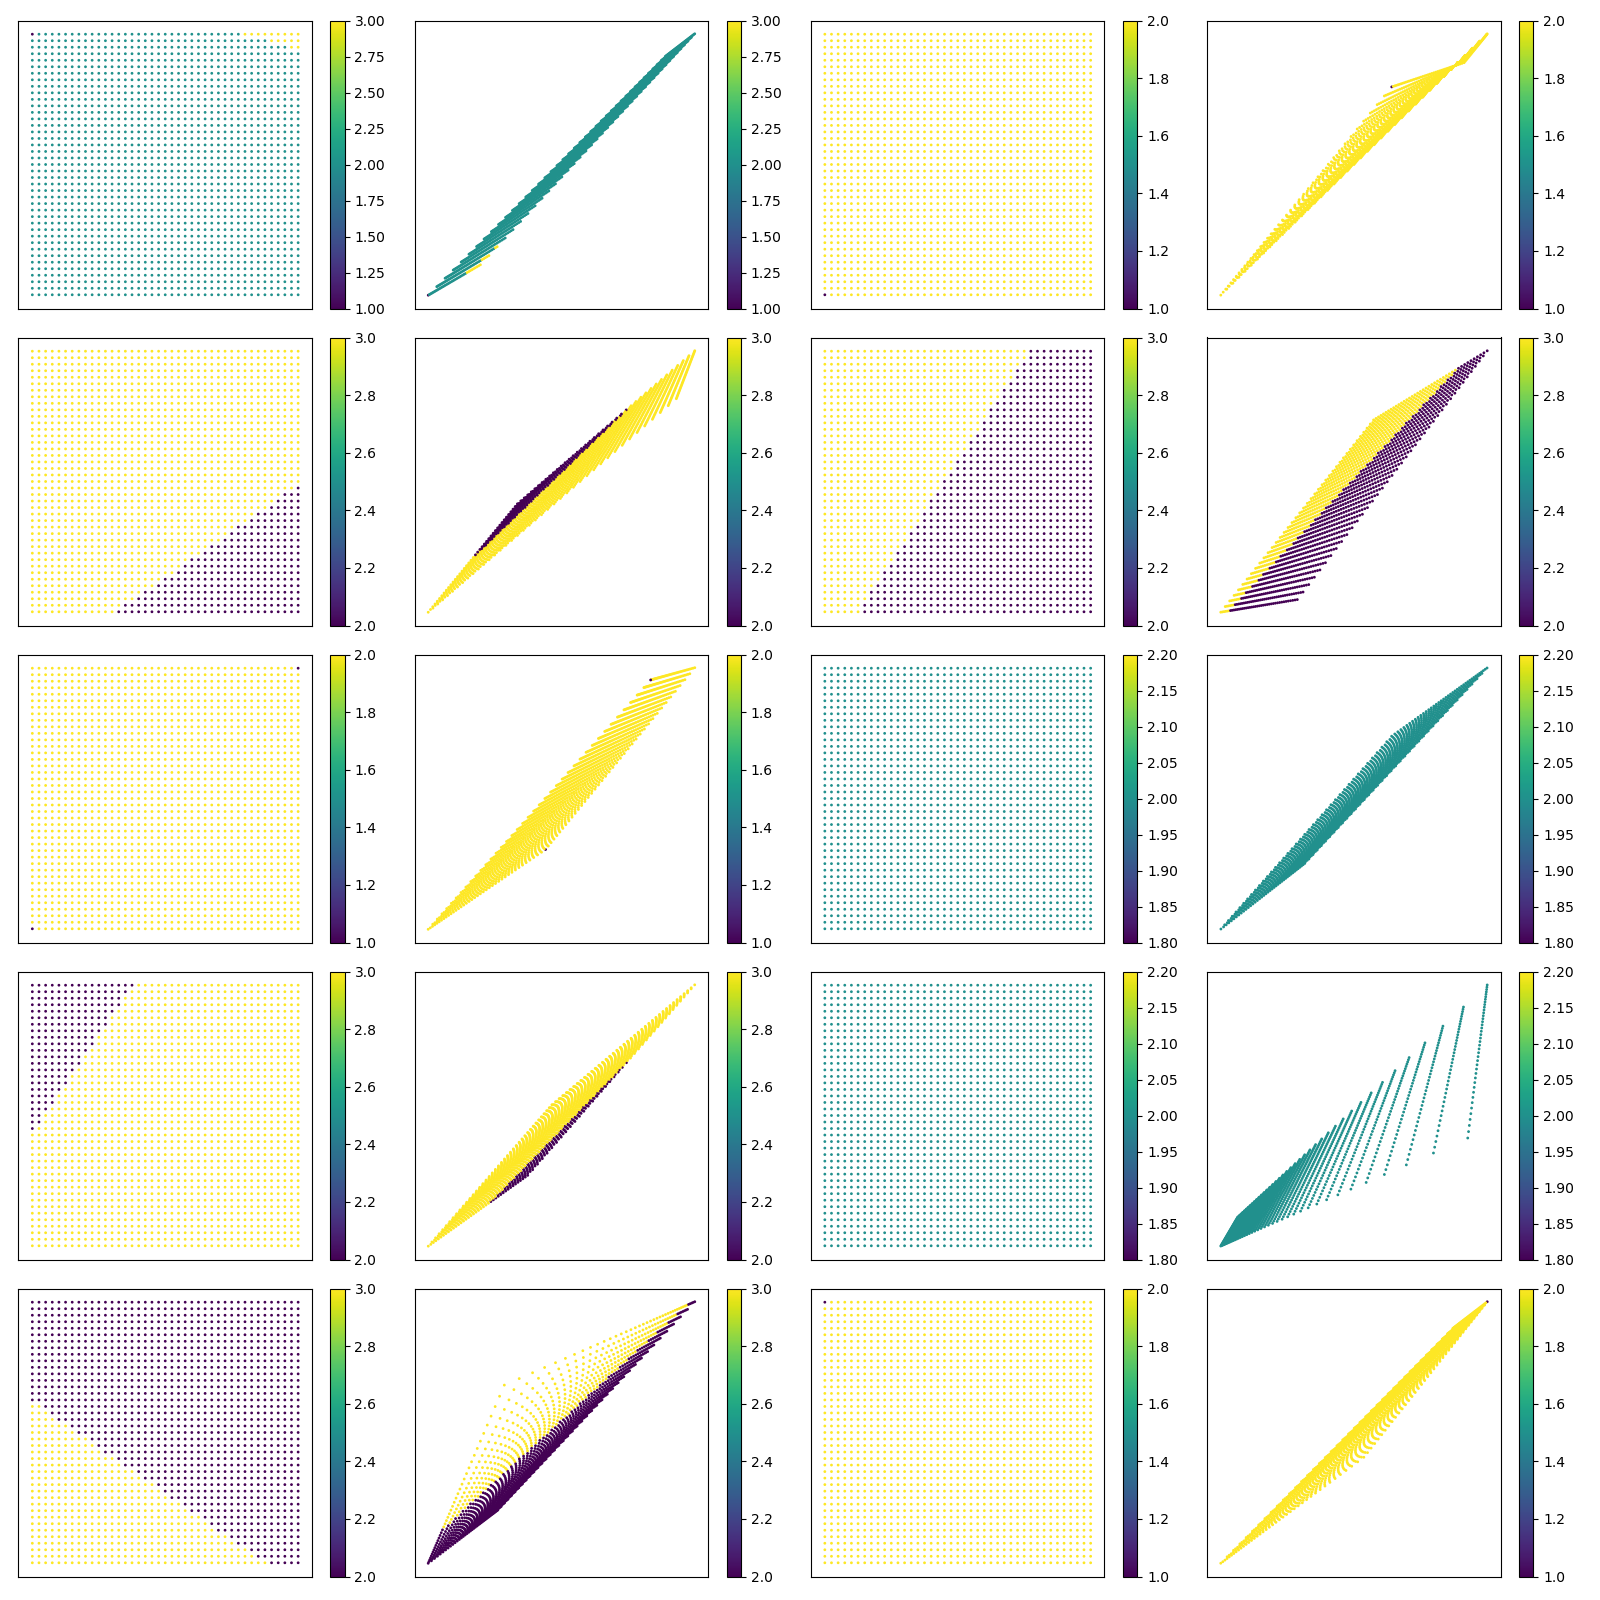
\includegraphics[width=0.5\textwidth,height=0.5\textheight]{../../pictures/figures/gpi-partitions.png}
\caption{`2-state 2-action MDPs. We have visualised the number of steps
required for convergence to the optimal policy. The number of steps are
show by color.'}
\end{figure}

\begin{itemize}
\item
  \textbf{Observation} Two policies can be within \(\epsilon\) yet
  requires more iterations of GPI. \textbf{Question} Why are some
  initial points far harder to solve than others, despite being
  approximately the same?
\item
  \textbf{Observation} With only 2 states and 2 actions, it is possible
  for 3 partitions to exist. (2,3,4 steps), (2,3,2 steps).
  \textbf{Questions} ???
\item
  \textbf{Observation} Sometimes the iterations don't converge. (a bug
  in the code?)
\end{itemize}

NOTES:

\begin{itemize}
\item
  What are the best ways to travel through policy space? (lines of
  shortest distance?!)
\item
  How does this scale with \texttt{n\_actions} or \texttt{n\_states}??
\item
  Is there a way to use an interior search to give info about the
  exterior? (dual methods?!)
\item
  What if your evaluations are only \(\epsilon\)-accurate? How does that
  effect things?!?
\end{itemize}reater pleasures, or else he endures pains to avoid worse pains.''

\subsection{Search spaces and gradient descent}

We want to find the optimal policy given some MDP. But how should we
search for this policy? We could search within set of potentially
optimal policies, the \(|A|^{|S|}\) discrete policies, or we could
search within the set of possible value functions, \(\mathbb R^{|S|}\),
or maybe some other space. Which space allows us to find the optimal
policy in the cheapest manner?

Naively, we know that smaller search spaces are better. We would rather
search for our keys in a single room, rather than many. But added
structure (for example, continuity) can be exploited to yield faster
search, even when there are infinitely more states to search.

In RL we know that; - the values must satisfy the bellman optimality
criteria. This structure can be exploted. - the policies \ldots{}?

\paragraph{Value iteration}

In RL it is possible to transform the hard combinatorial problem of
searching through the \(|A|^{|S|}\) possible discrete policies, into an
easier (how do we know it is easier?!? PROOF) problem, a search through
all possible policies \(?!?\).


\paragraph{Policy iteration}

When transforming between two spaces, how does the optimisation space
change? Does my abstraction make optimisation easier?


\paragraph{Model iteration}

Search through possible models, \(\tau, r\), calculate the optimal
policy \(\pi^{* }_{\tau, r}\) and then update \(\tau, r\) based on
\(\parallel V_{\tau, r}(\pi^{* }) - V(\pi^{* }) \parallel\).

Search through models while trying to find one that yields similar returns to the oracle when playing the same policy.
A supervised problem...

\begin{align}
\theta^{* } = \mathop{\text{argmin}}_{\theta} \int_{\Pi} \parallel V^{\pi}_{P, r} -V^{\pi}_{\theta} \parallel_2
\end{align}

Note this solver is different to the others. In the previous optimisations we assumed that we knew the model.

% Related to;
% - Thompson sampling?!?
% - invaraint risk minimisation
% - compressed sensing. each policy is one of our sampling bases!? rather than using the deterministic policies (the pixels), we can use mixtures!?

Once we have the model, we can solve for the optimal policy.

Relation to model based RL. This algol only focuses on relevant features of the state space.
Where model base learners that attempt to learn by predicting transitions can be made to scale arbitrarily worse.
Consider a problem where the reward is only determined by the first feature of the state. We can add $n$ extra, useless, features.
The model based learner will spend resources on attempting to build a good predictor of those $n$ features.

Sample efficient. You only need to collect data for the $m$ policies we are matching under.
Once that has been done, the optimisation problem is easily solved!?

Model iteration. Model invariant transforms. Pick a policy. Falsify it,
and this falsify all models that yield the same optimal policy.

\begin{figure}
\centering
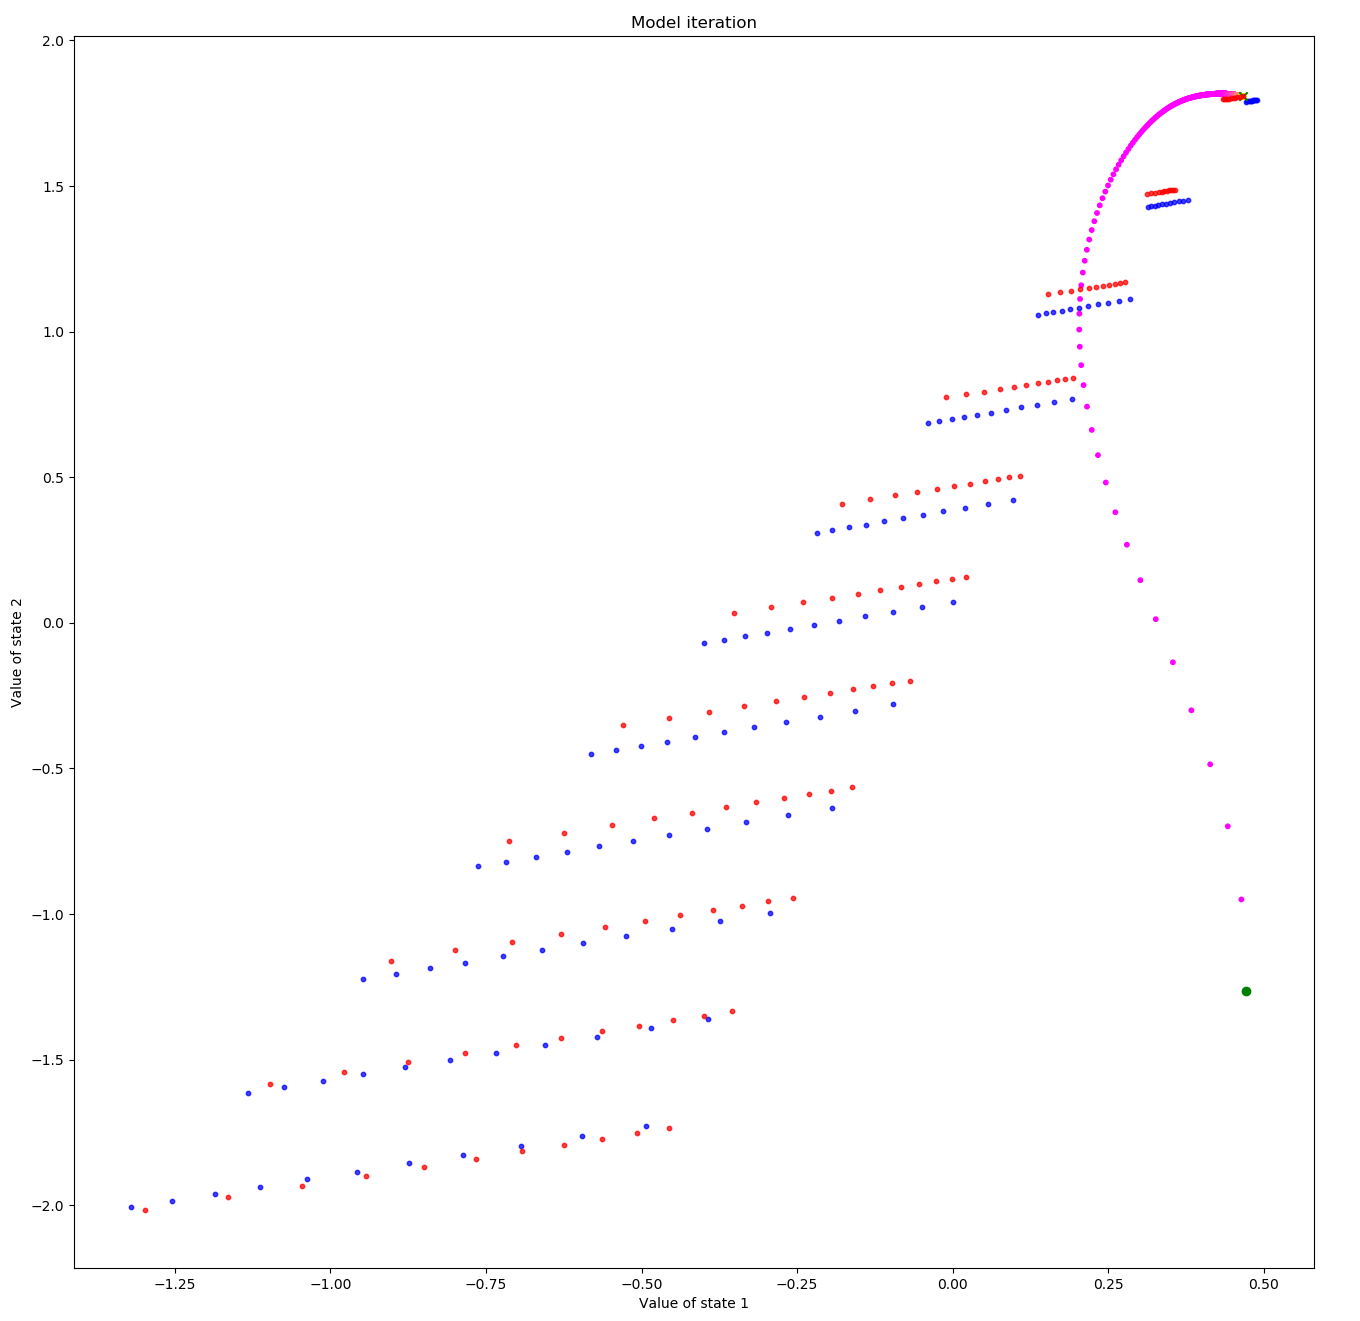
\includegraphics[width=0.5\textwidth,height=0.5\textheight]{../../pictures/figures/model_iteration.png}
\caption{Blue shows the value of policies when evaluated under the true model, $P, r$,
and Red shows the value of policies when evaluated under the learned model at convergence.}
\end{figure}

\begin{center}\rule{0.5\linewidth}{\linethickness}\end{center}

More generally, I am interested in how searches in different spaces,
whether the value, the policy, or some parameters, \ldots{}

Let's focus on gradient descent.

\begin{align}
w_{t+1} = w_t - \eta \nabla f(w_t) \\
\end{align}

It's dynamics are depentdent on the topology of its loss landscpace,
which is determined by the search space and .

Thus phrased differently, the original becomes: how does the space we
are searching within effect the search dynamics: the rate of convergence
and the possible trajectories.

\begin{align}
&\mathop{\text{max}}_V \mathop{\mathbb E}_{s\sim D} V(s) \\
&\mathop{\text{max}}_{\pi} \mathop{\mathbb E}_{s\sim D}V^{\pi}(s) \\
&\mathop{\text{max}}_{\theta} \mathop{\mathbb E}_{s\sim D} V_{\theta}(s) \\
&\mathop{\text{max}}_{\theta} \mathop{\mathbb E}_{s\sim D} V^{\pi_{_{\theta}}}(s) \\
&\mathop{\text{max}}_{\phi} \mathop{\mathbb E}_{s\sim D} V^{\pi_{_{\theta_{\phi}}}}(s) \\
&\mathop{\text{max}}_{\varphi} \mathop{\mathbb E}_{s\sim D} V^{\pi_{_{\theta_{\phi_{\varphi}}}}}(s) \\
\end{align}

We could pick any space we we like to search with in. But, why would we want to pick one space over another?

\begin{itemize}
\tightlist
\item
  In which spaces can we efficiently do gradient descent?
\item
  In which spaces can we do convex optimisation?
\item
  In which spaces does momentum work well?
\end{itemize}

\subsubsection{Topology and dynamics}

Ok, so if we parameterise our search space. We have now changed the
topology of our search space.

\textbf{Q:} How can we rationally pick the topology of our search space
to accelerate learning?

\begin{itemize}
\item
  A well connected space? For all possible policies, there exists
  \(\theta_1, \theta_2 \text{ s.t. } \parallel \theta_1- \theta_2\parallel_2\)
  is small. (but that doesnt necessarily help\ldots{} depends on the
  landscapce imposed by \(\nabla_{\theta} V\))
\item
  ???
\end{itemize}

See these gradient flows for example;

Pics?!?

Here are some examples \ldots{}???

\begin{figure}
\centering
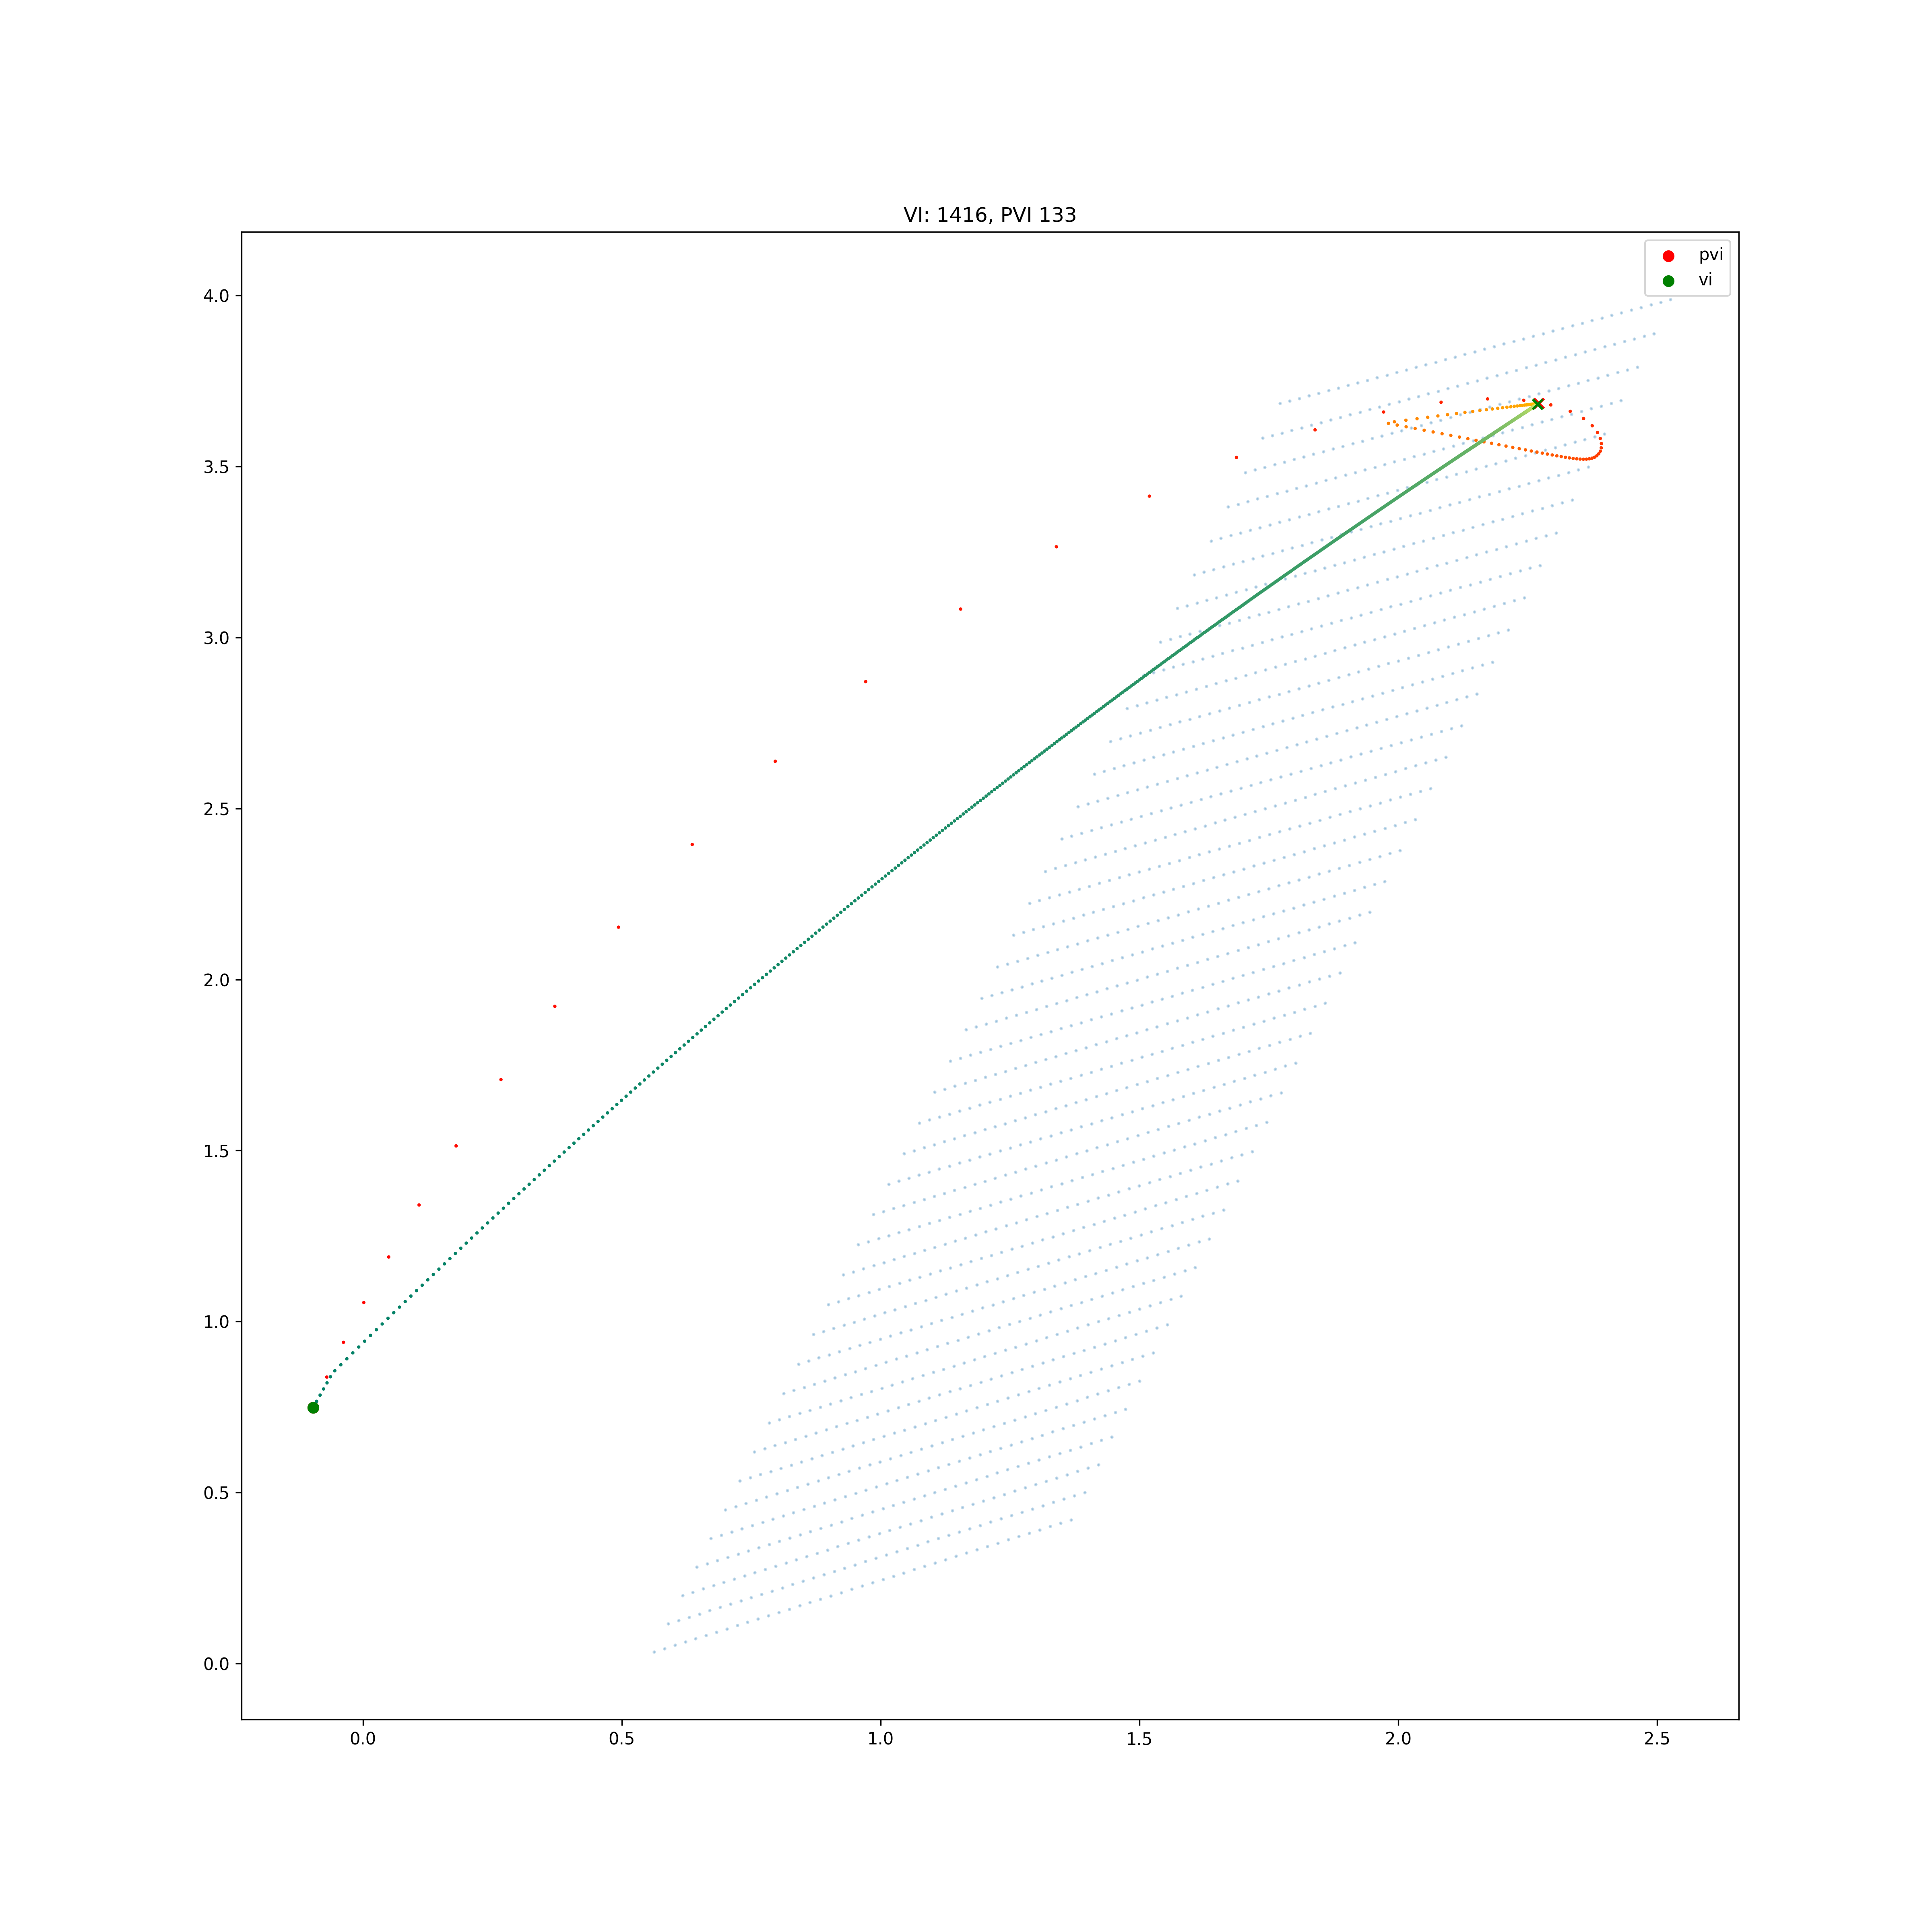
\includegraphics[width=0.5\textwidth,height=0.5\textheight]{../../pictures/figures/vi-vs-pvi.png}
\caption{The optimisation dynamics of value iteration versus parameterised value iteration.}
\end{figure}

\begin{figure}
\centering
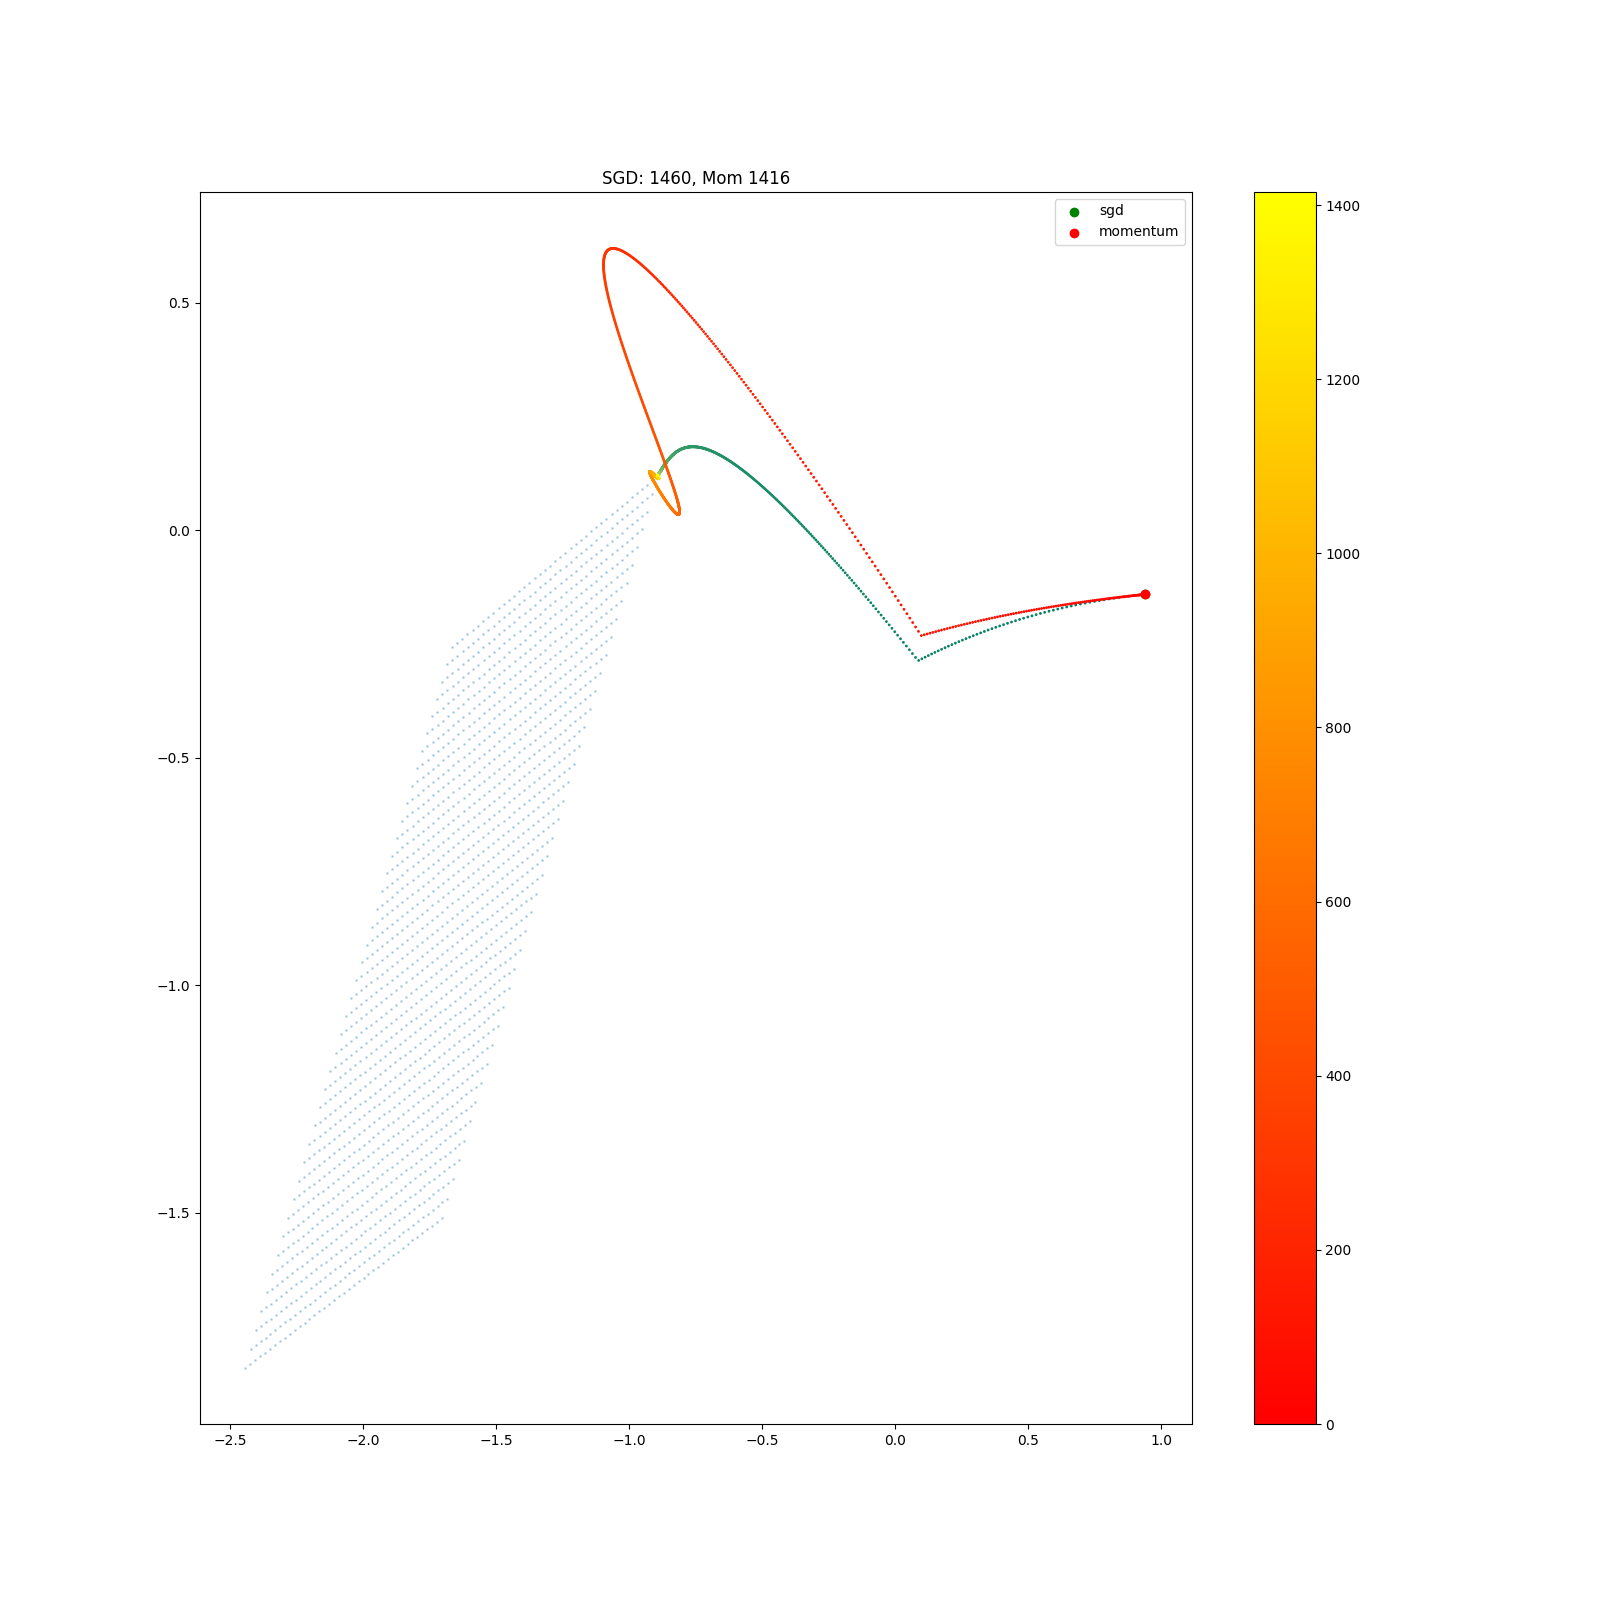
\includegraphics[width=0.5\textwidth,height=0.5\textheight]{../../pictures/figures/vi_sgd-vs-vi_mom.png}
\caption{The optimisation dynamics of value iteration versus value iteration with momentum.}
\end{figure}

If we overparameterise the search space, then we can move between solutions in new ways. We can `tunnel' from A to B, without crossing C.
%  insert pic / prove

Every point (in output space) is closer, when measured in the distance in parameter space needed to be traveled.
% insert pic / prove


\subsubsection{Accleration and parameterisation}

I think something weird happens with momentum in overparameterised spaces. The intuition is

We have implicit momentum from the parameterisation, and explicit momentum in the accelerated descent.

It is necessary to consider the trajectory to study momentum. It depends
on what has happened in the past. Can we construct a space of possible
trajectories? What properties do trajectories have? They are connected
by the update fn.


\subsubsection{Continuous flow and its discretisation}

A linear step of size, \(\alpha\), in parameter space, ie by gradient
descent, is not necessrily a linear step in parameter space.

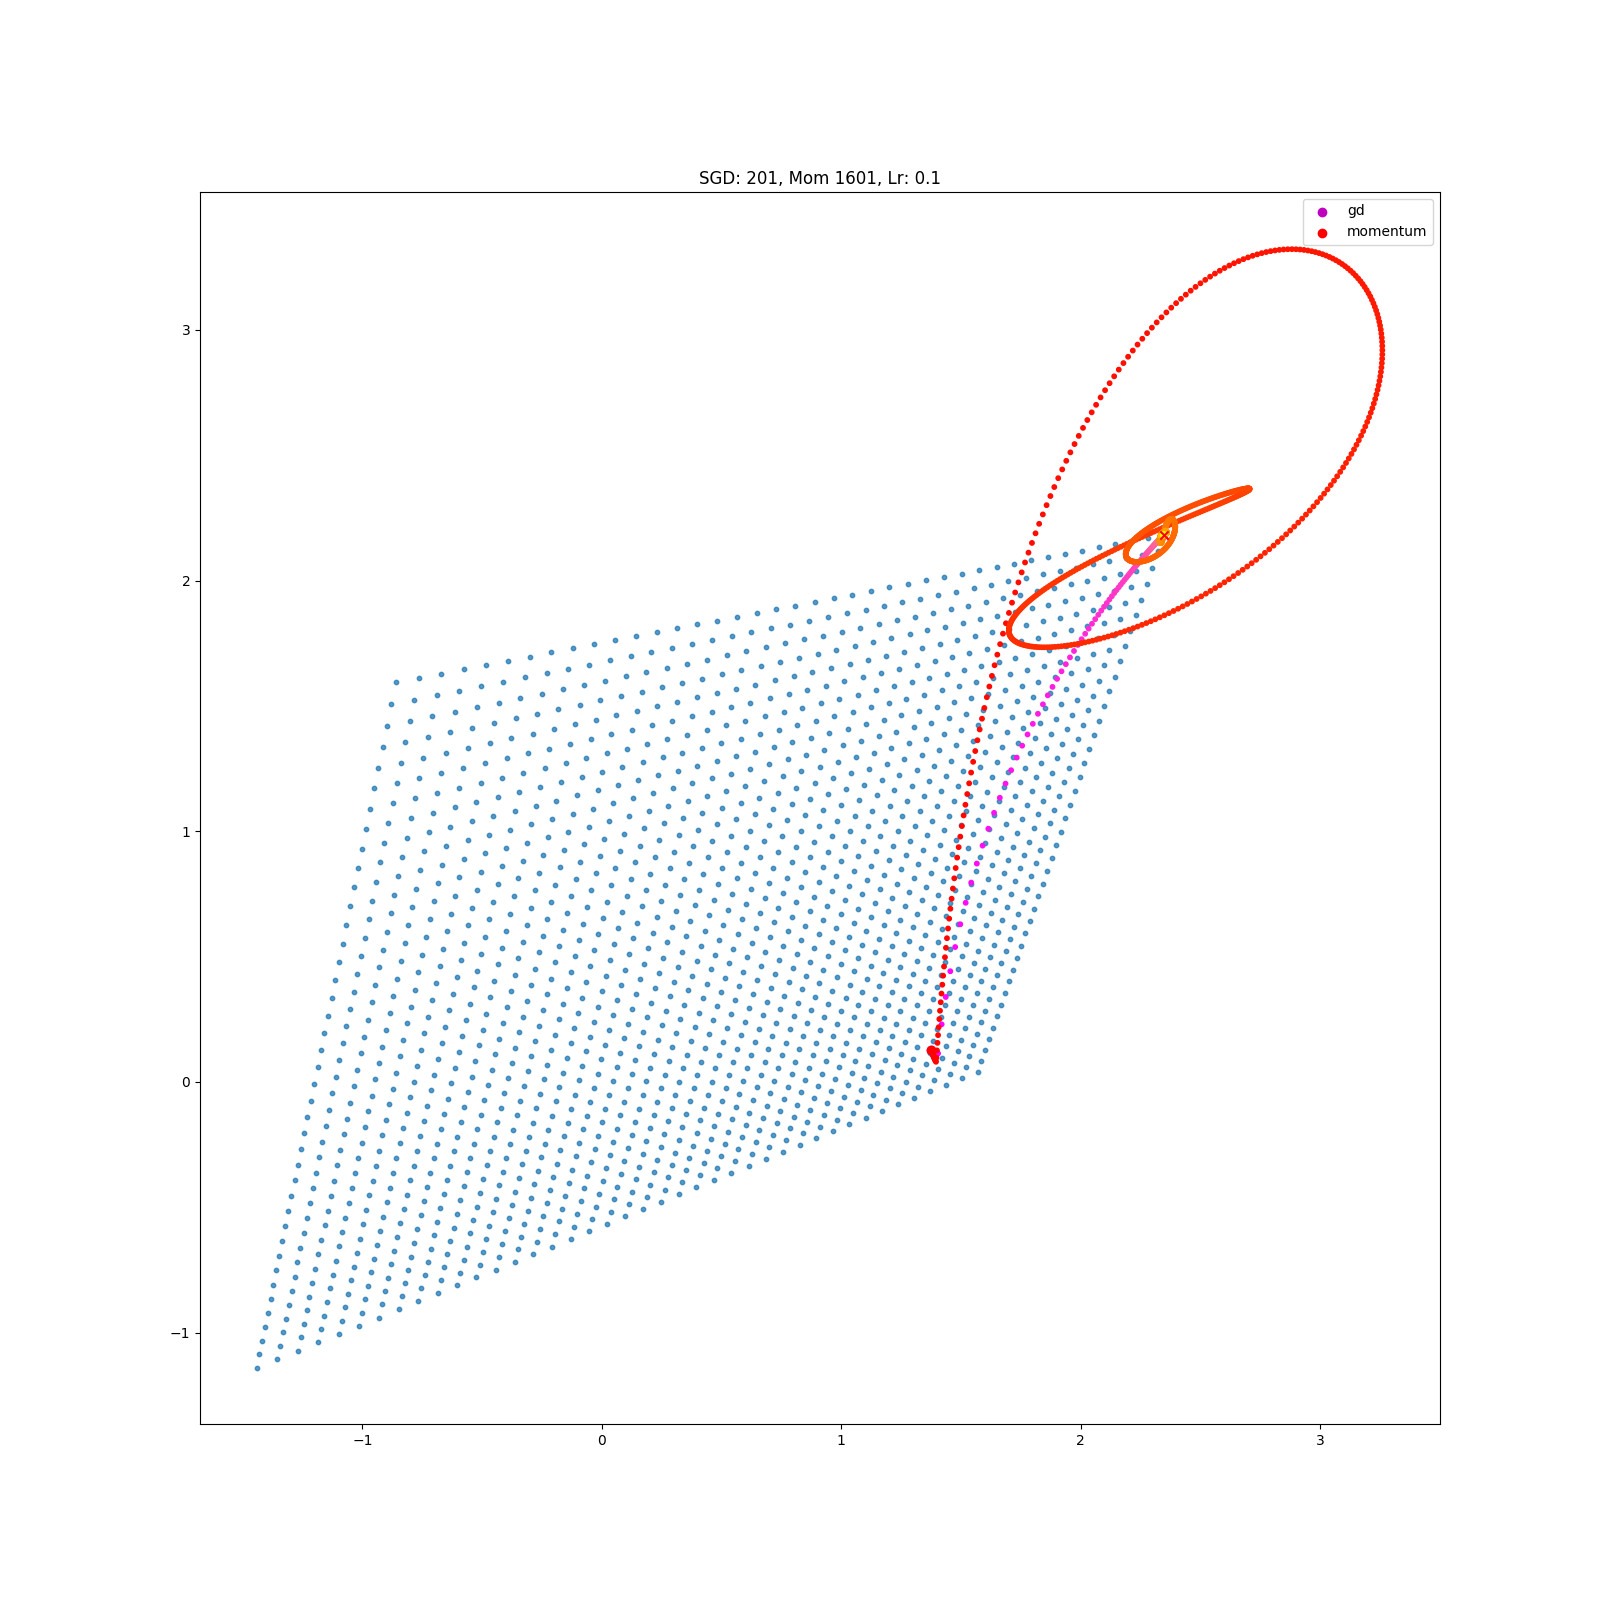
\includegraphics[width=0.5\textwidth,height=0.5\textheight]{../../pictures/figures/vi_sgd-vs-vi_mom_01.png}
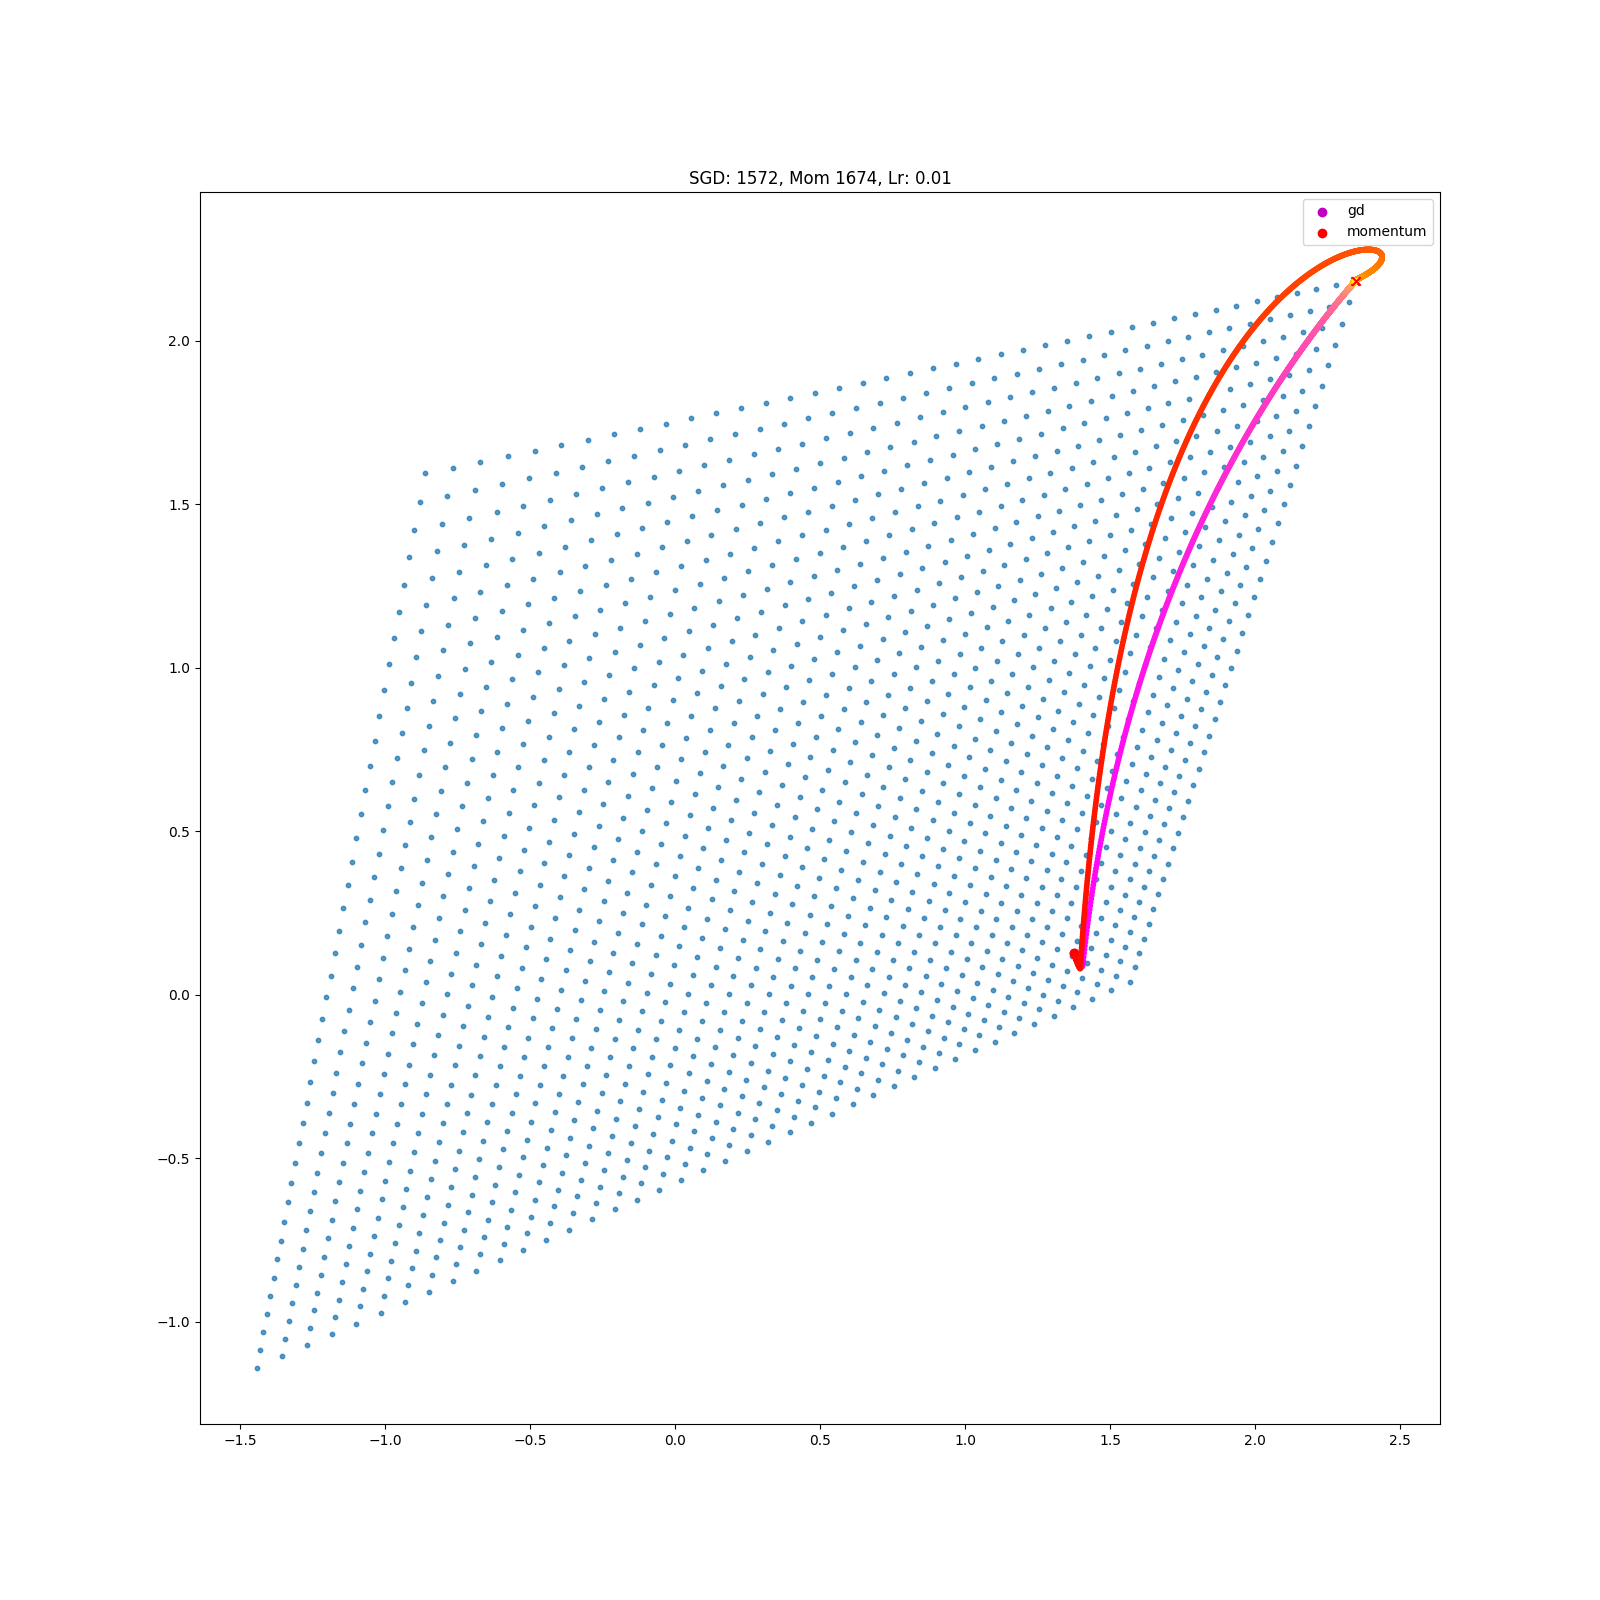
\includegraphics[width=0.5\textwidth,height=0.5\textheight]{../../pictures/figures/vi_sgd-vs-vi_mom_001.png}
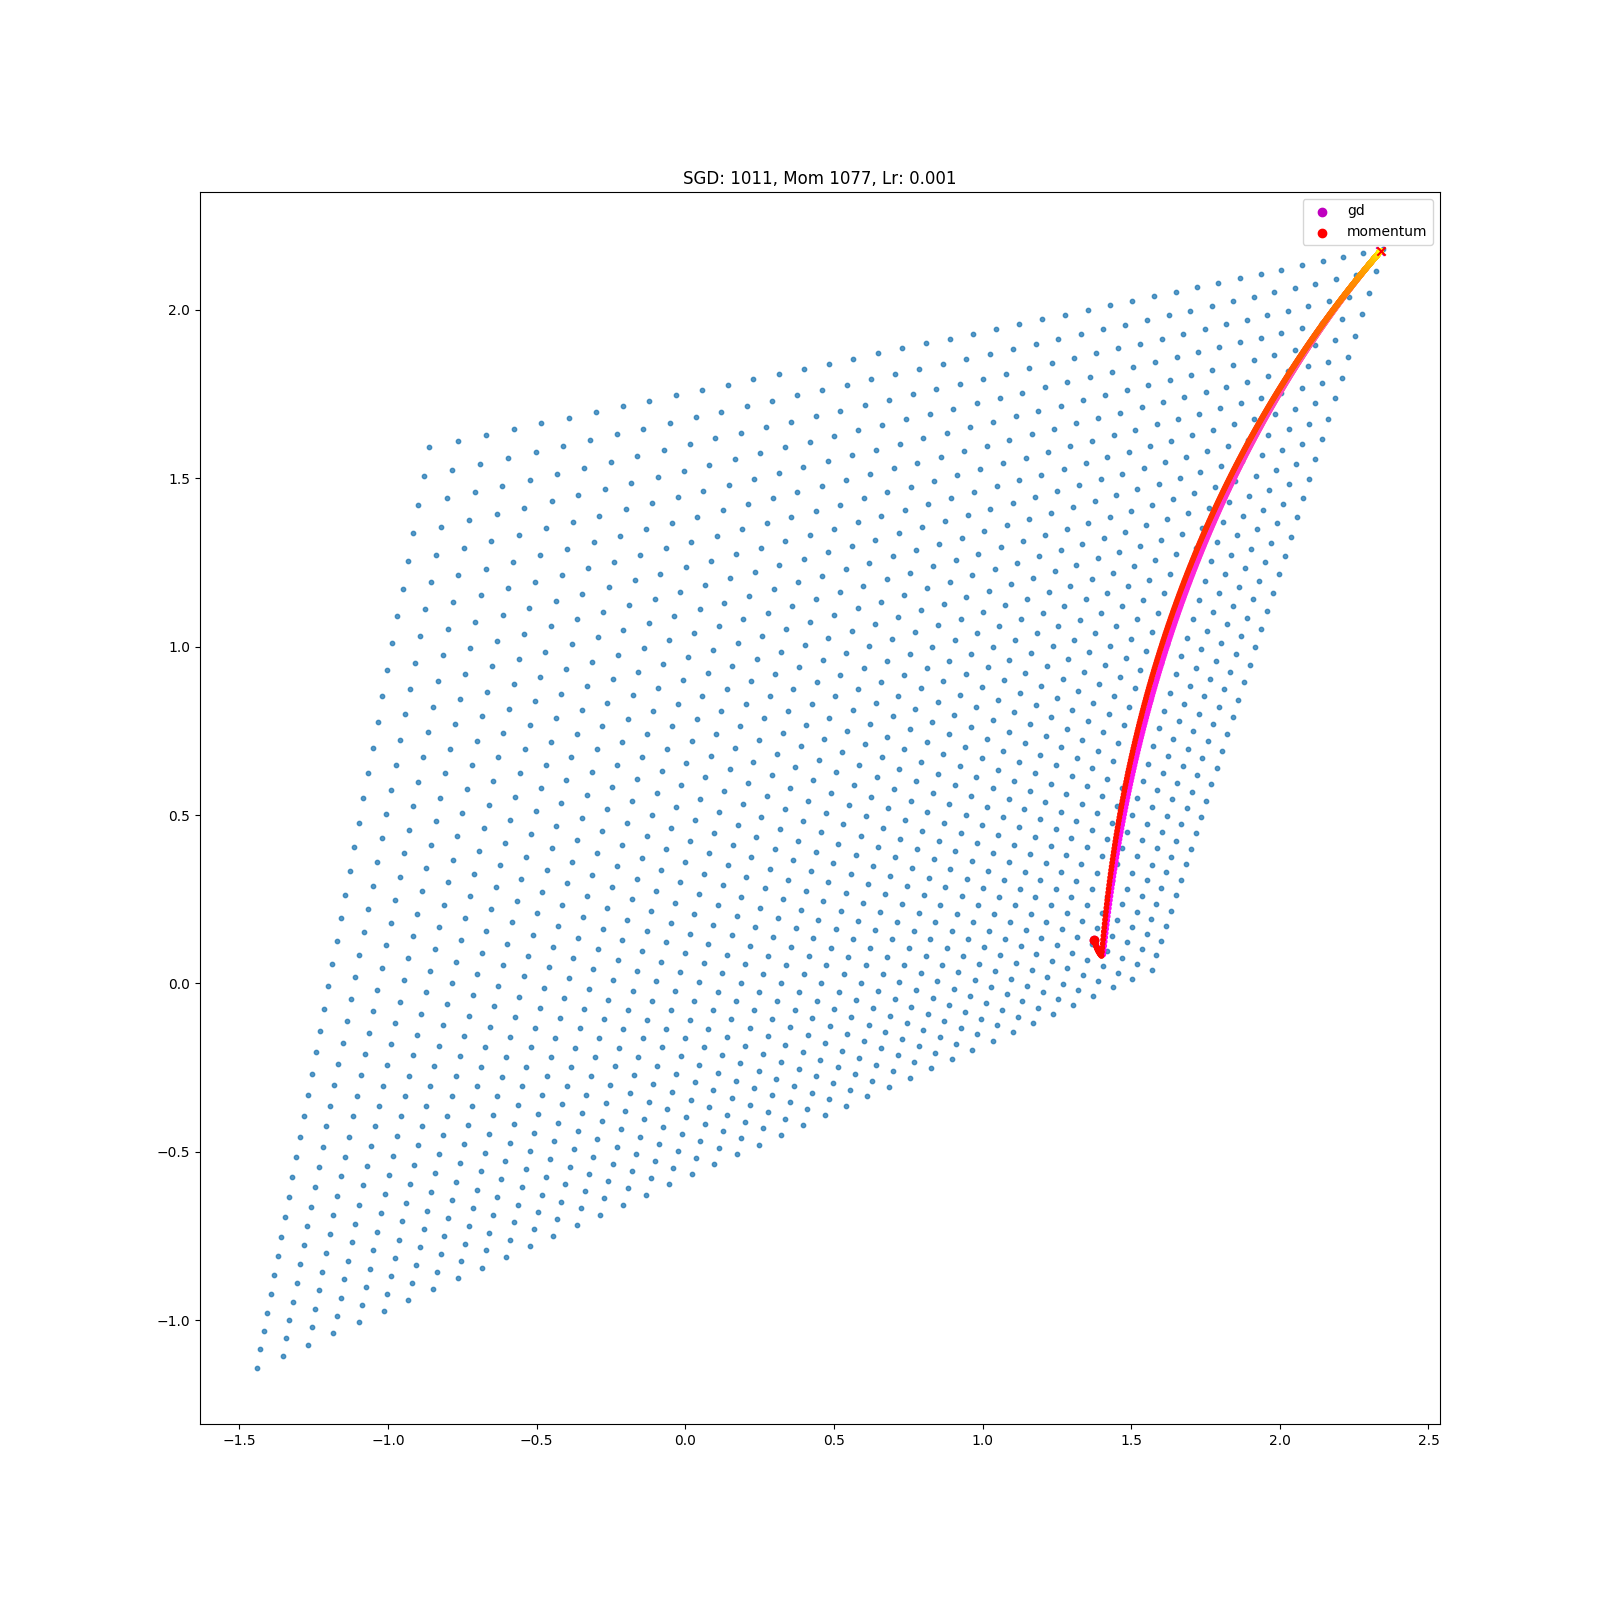
\includegraphics[width=0.5\textwidth,height=0.5\textheight]{../../pictures/figures/vi_sgd-vs-vi_mom_0001.png}

This is consistent with acceleration of gradient descent being a phenomena only possible in the discrete time setting. (see \cite{Betancourt2018} for a recent exploration)

This phenomena can be explained by the exponential decay of the momentum terms.

\begin{align}
m_{t+1} = m_t + \gamma\nabla f(w_t) \\
w_{t+1} = w_t - \eta (1-\gamma) m_{t+1} \\
\end{align}

As \(\eta \to 0\), \((1-\gamma) \cdot m_{t+1} \to \nabla f(w_t)\).

TODO, prove it.
